\newpage
\setcounter{secnumdepth}{1}
\section{Behavior analysis of Bush-Mosteller lineal and incremental learning algorithms}

\subsection{The Linear BM model}
$$f_{ij}(k+1) =α f_{ij}(k)  + (1-\alpha) \beta (k)$$ where $0 \leq \alpha \leq 1$  is the learning ratio and $\beta$(k) stands for the reward function associated with  the current  $k$-th exploration such that $\alpha$(k)=1 for a reward.


\subsubsection{Binary}

\begin{figure}[ht]
\centering
\subfigure[Fitness evolution]{
	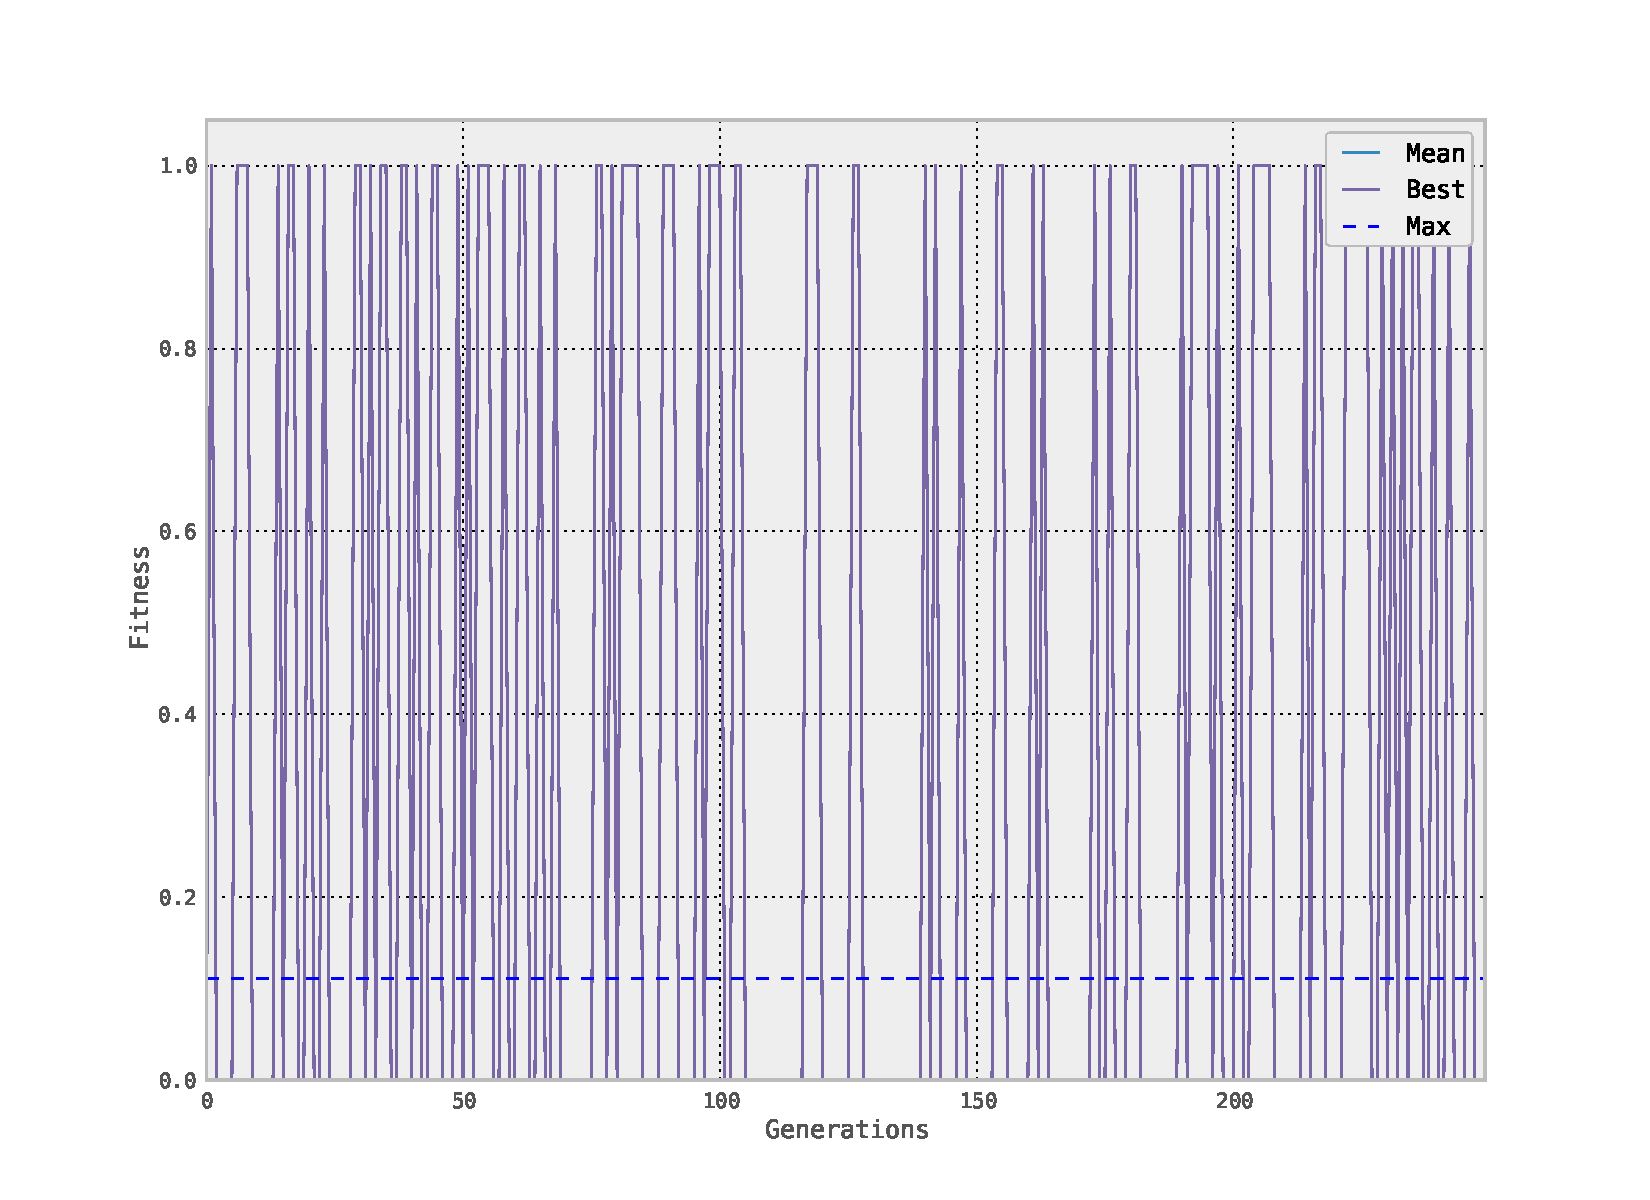
\includegraphics[scale =0.4] {images/section1/fitness_bush_mosteller_update_BinaryAnt.pdf}
	\label{fig:subfig11}
}
\subfigure[Pheromones per edge]{
	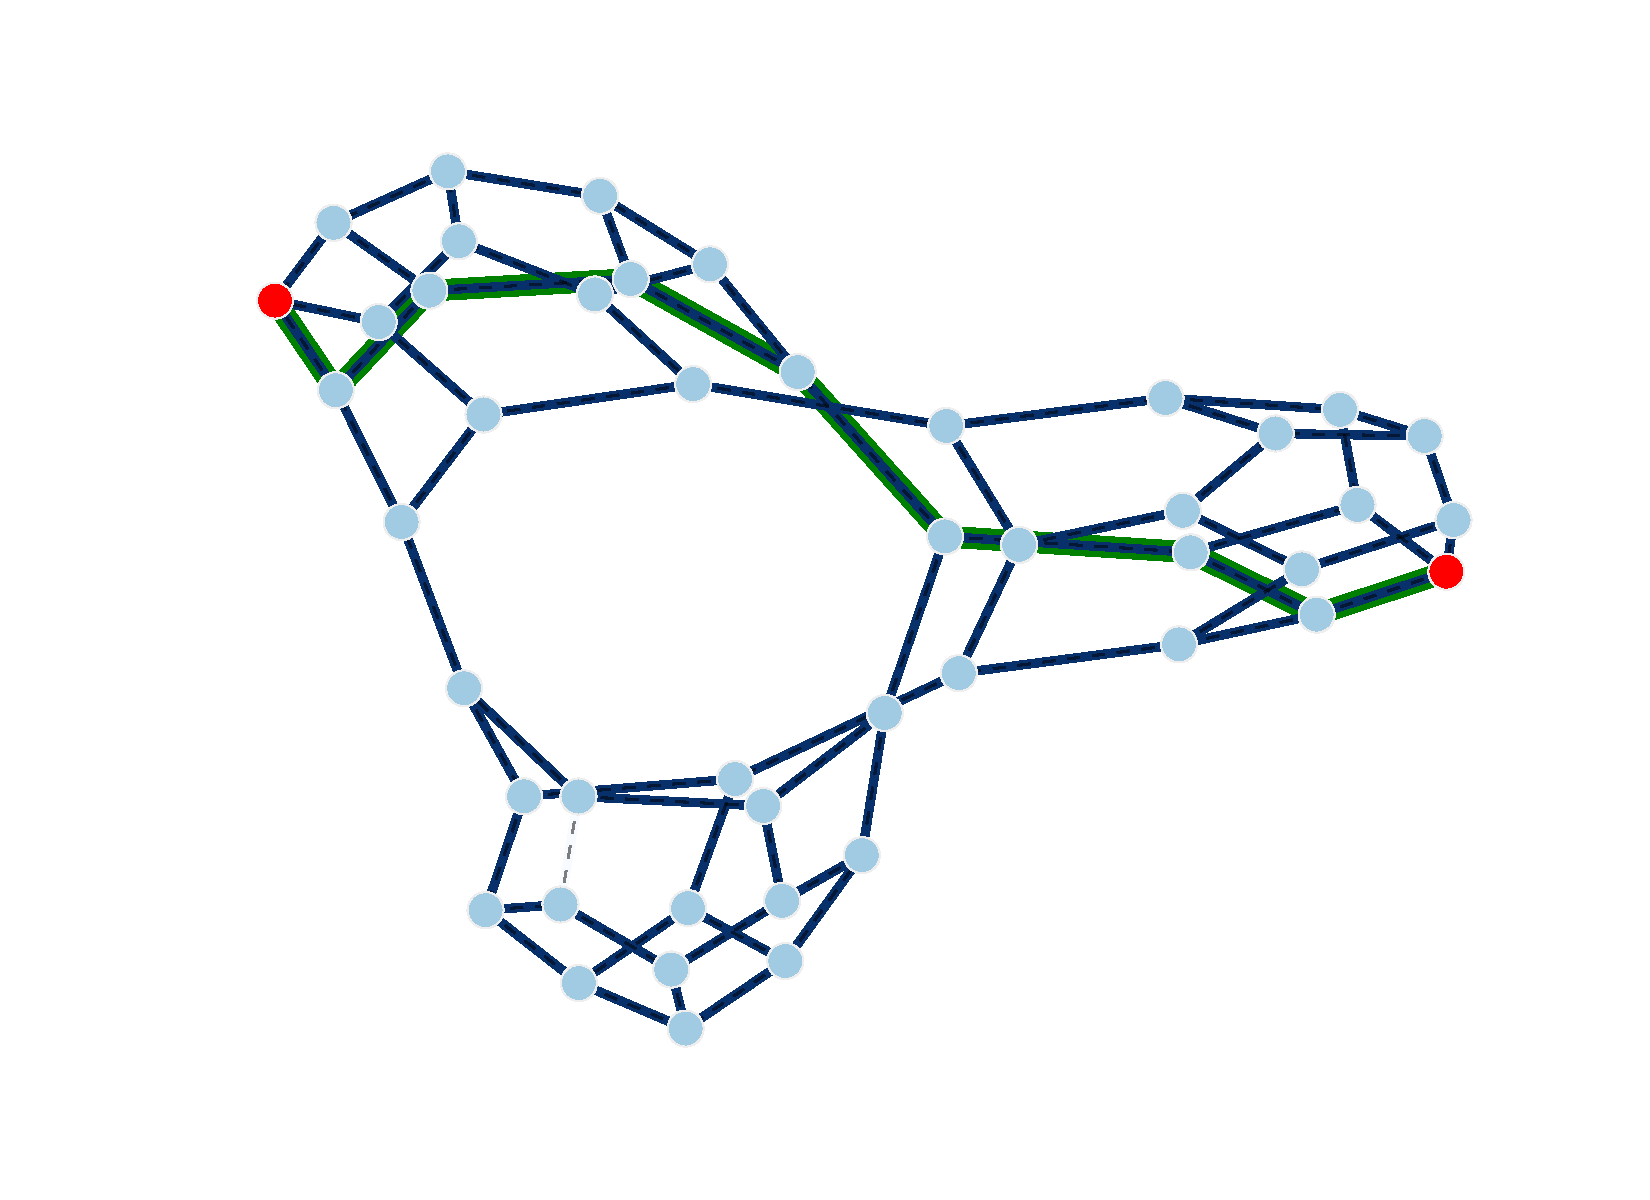
\includegraphics[scale =0.4] {images/section1/pheromones_bush_mosteller_update_BinaryAnt.pdf}
	\label{fig:subfig12}
}
%\caption[Optional caption for list of figures]{Caption of subfigures \subref{fig:subfig1}, \subref{fig:subfig2}}
\label{fig:fig1}
\end{figure}

\newpage
\subsubsection{Proportional}

\begin{figure}[ht]
\centering
\subfigure[Fitness evolution]{
	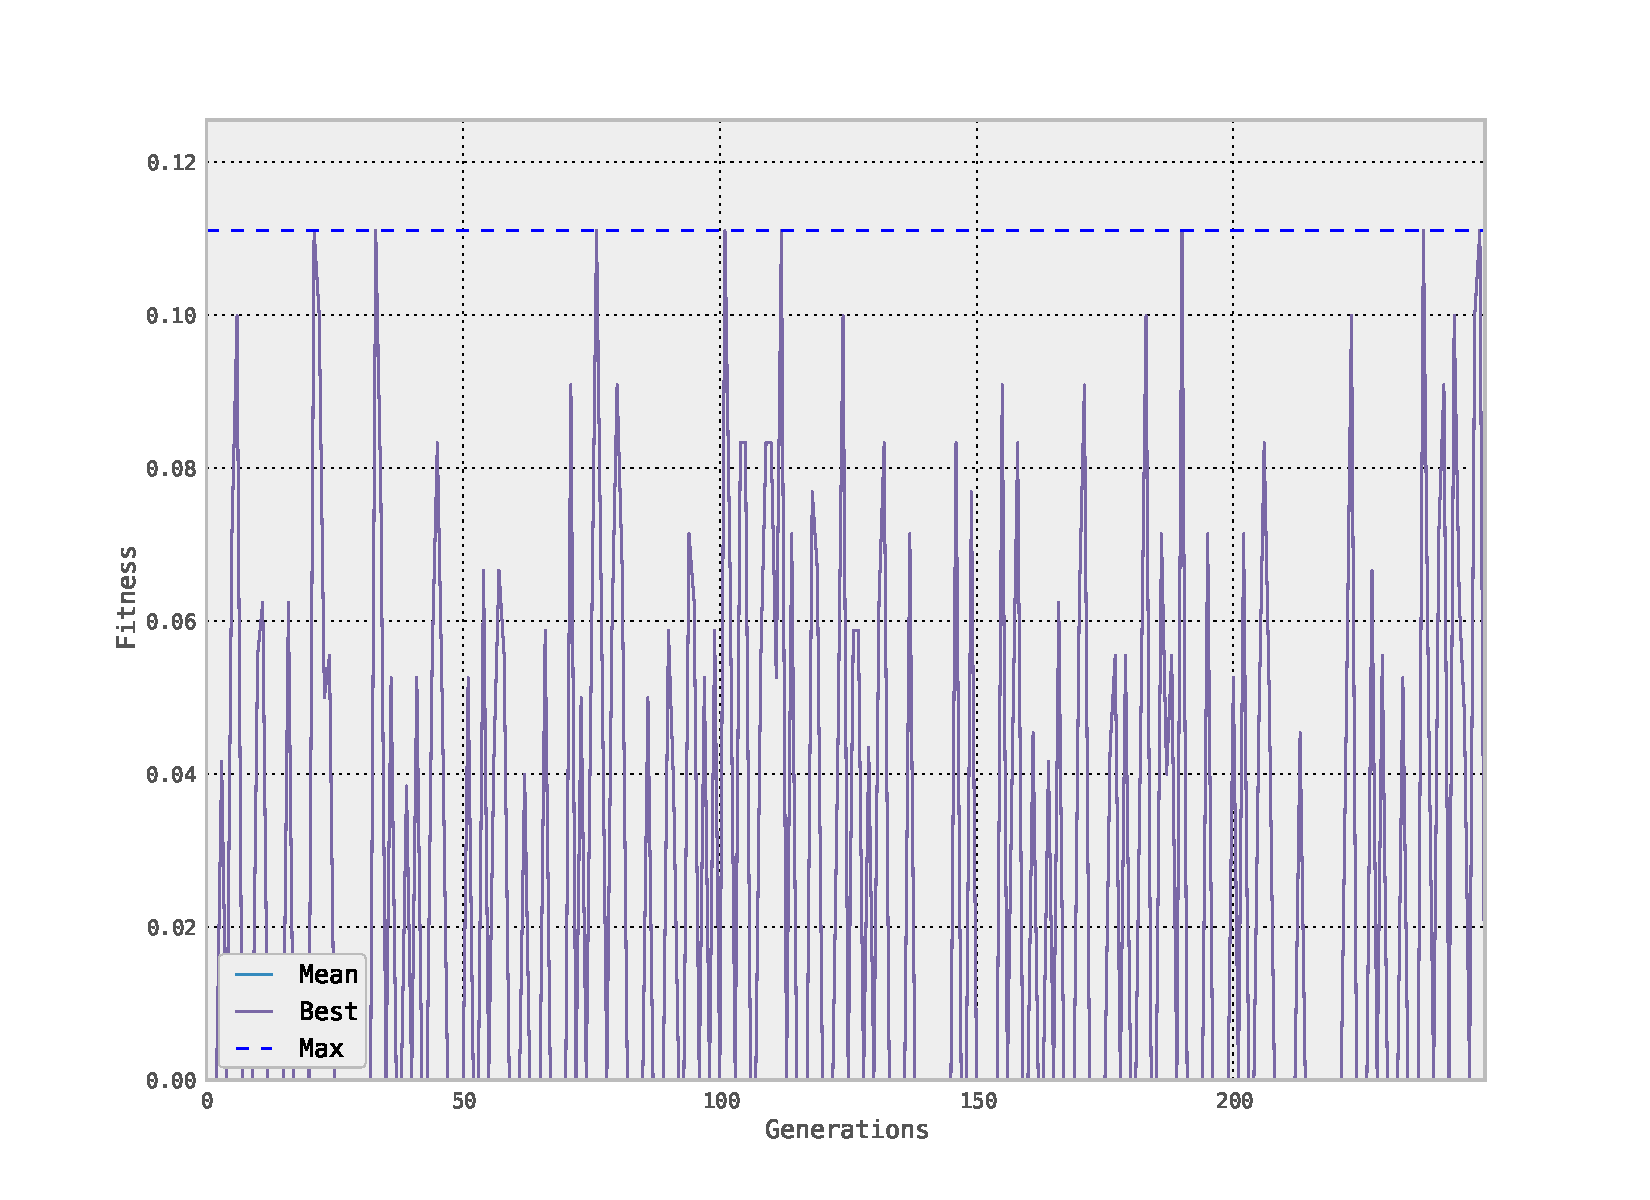
\includegraphics[scale =0.4] {images/section1/fitness_bush_mosteller_update_ProportionalAnt.pdf}
	\label{fig:subfig11}
}
\subfigure[Pheromones per edge]{
	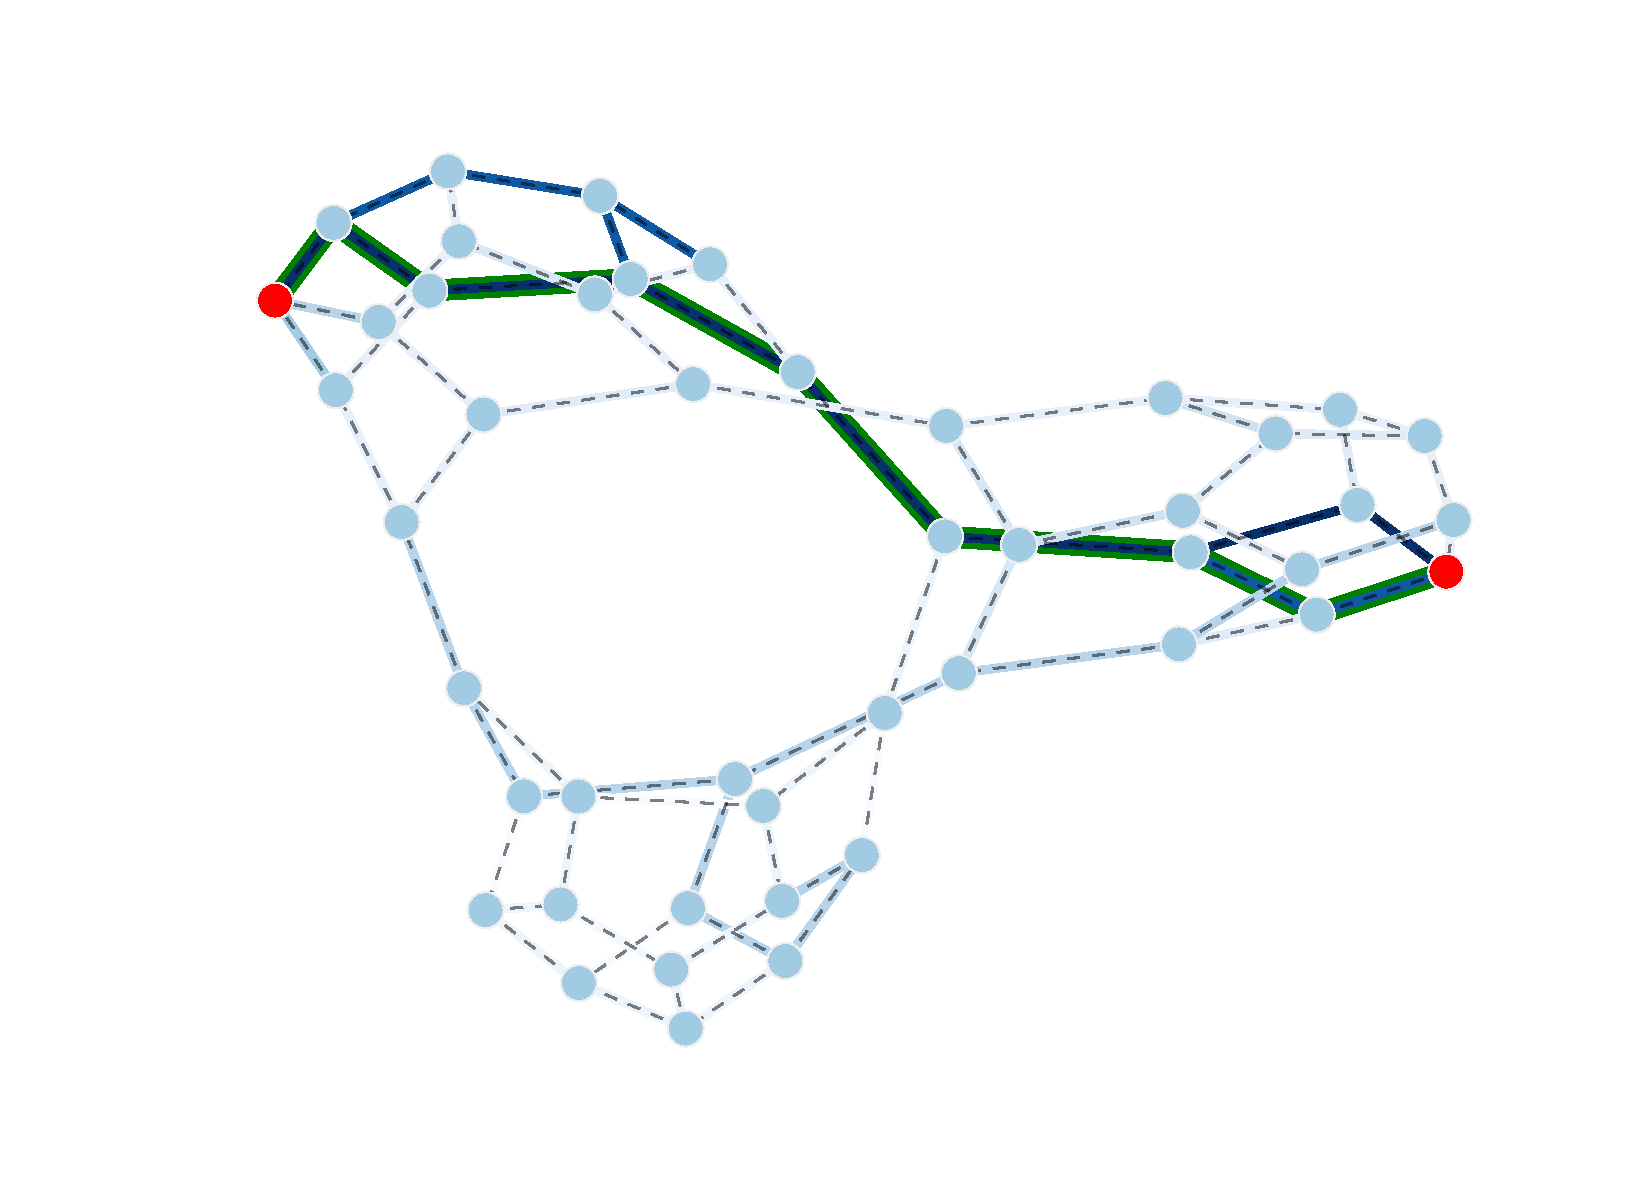
\includegraphics[scale =0.4] {images/section1/pheromones_bush_mosteller_update_ProportionalAnt.pdf}
	\label{fig:subfig12}
}
%\caption[Optional caption for list of figures]{Caption of subfigures \subref{fig:subfig1}, \subref{fig:subfig2}}
\label{fig:fig1}
\end{figure}














\newpage
\subsection{The incremental learning algorithm}
$$f_{ij} (k+1)   = f_{ij} (k) + \delta \beta(k)$$
where $0 \leq \delta \leq 1$ is the increment  design parameter and the reward signal $\beta$(k) has the same interpretation than in the previous algorithm.

\subsubsection{Binary}

\begin{figure}[ht]
\centering
\subfigure[Fitness evolution]{
	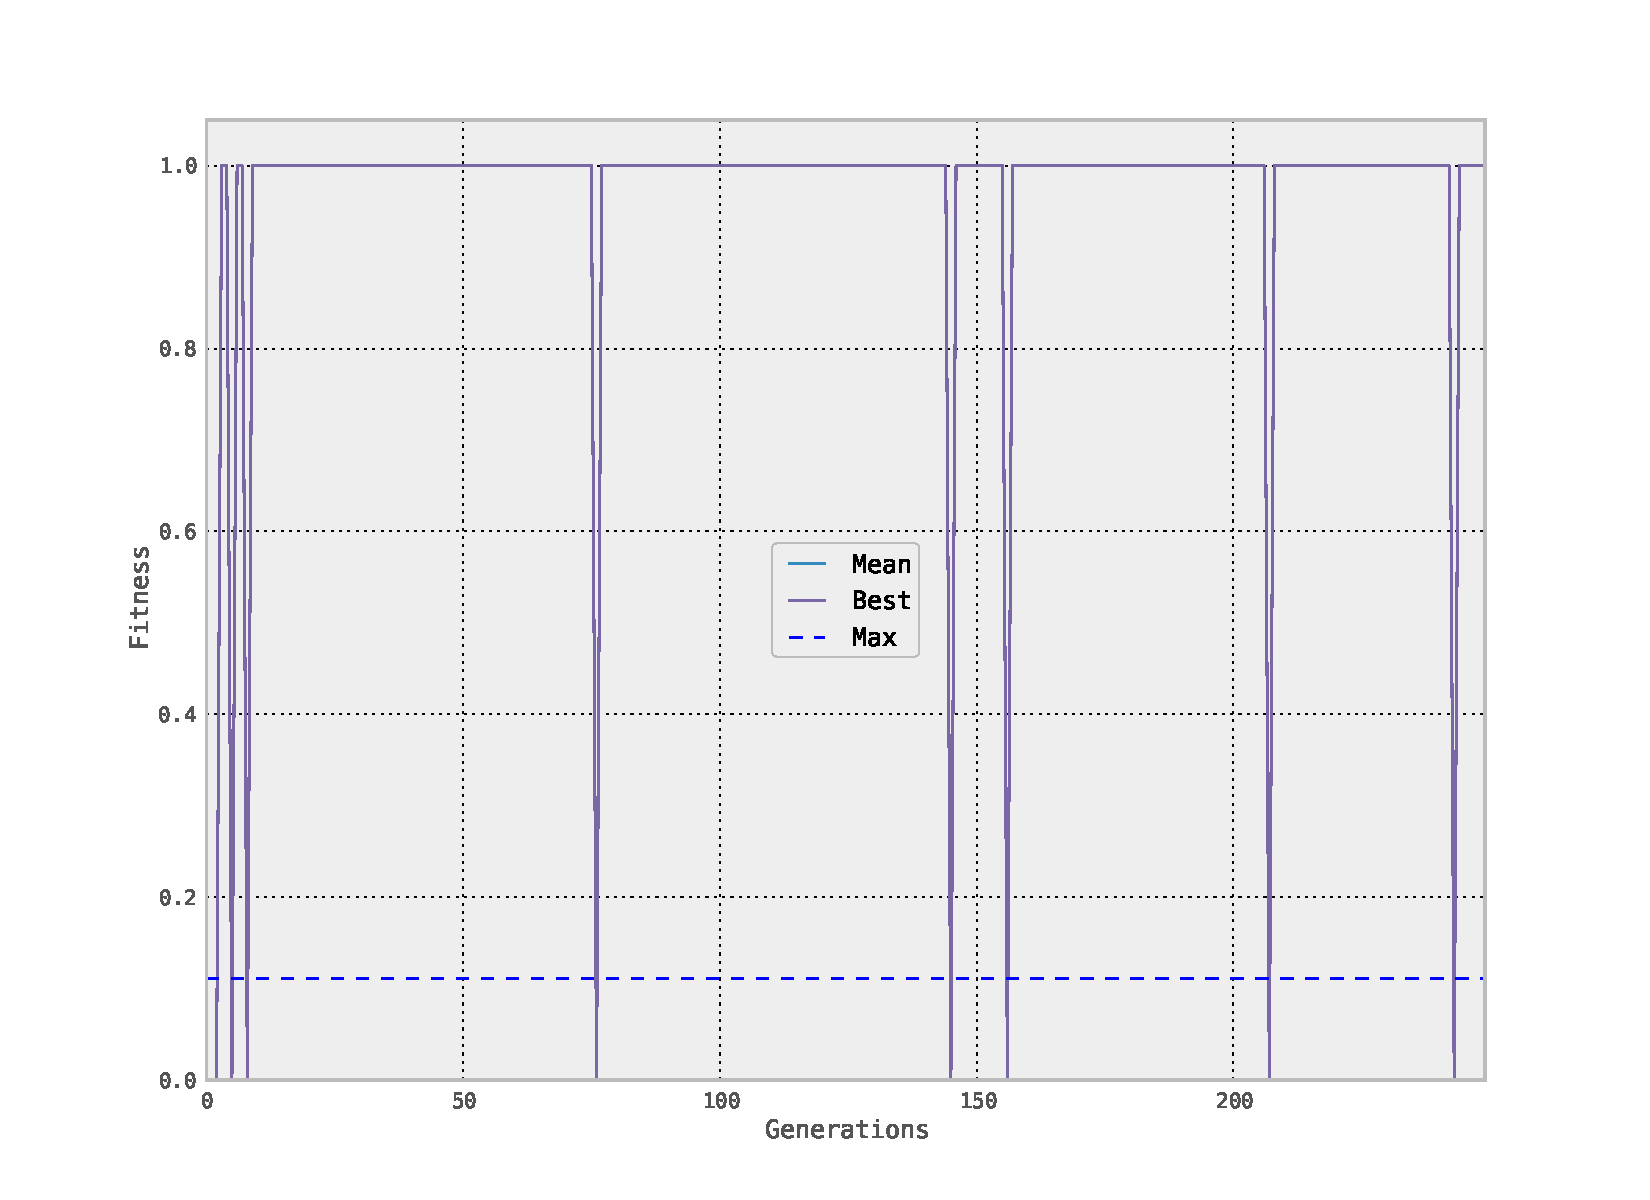
\includegraphics[scale =0.3] {images/section1/fitness_incremental_learning_update_BinaryAnt.pdf}
	\label{fig:subfig11}
}
\subfigure[Pheromones per edge]{
	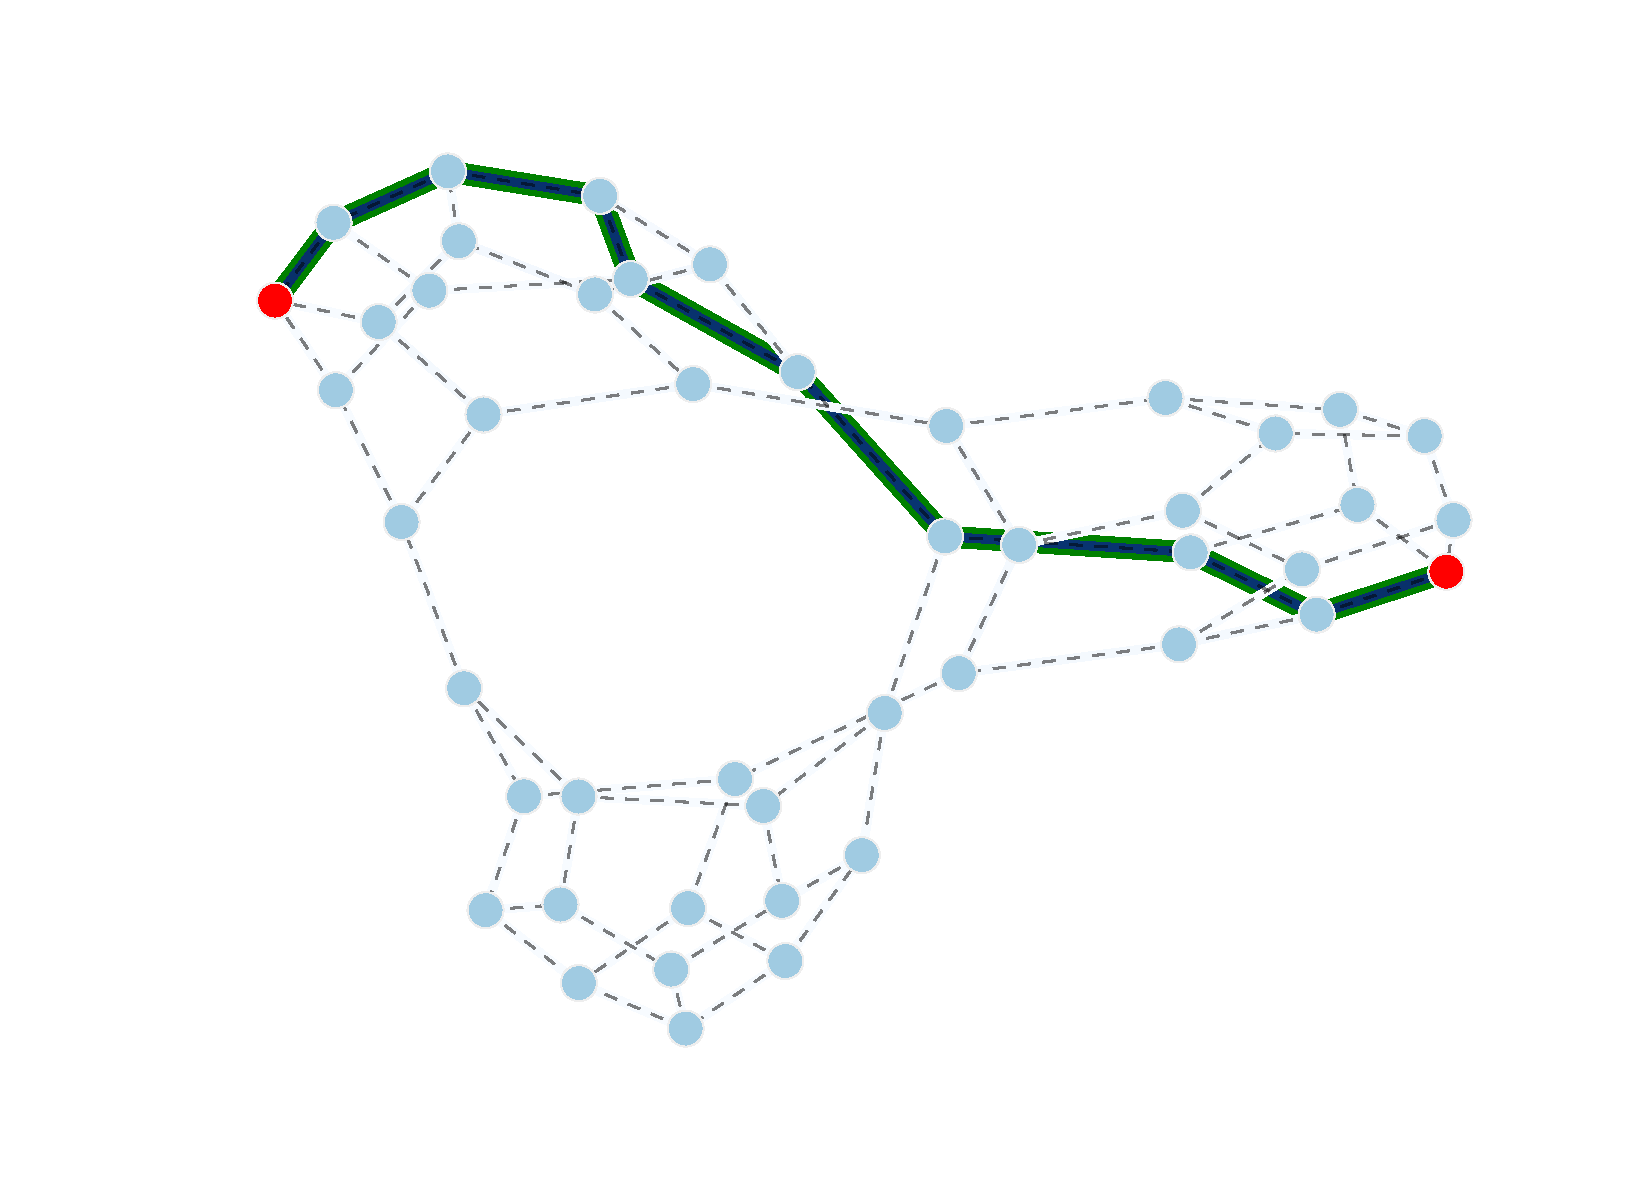
\includegraphics[scale =0.3] {images/section1/pheromones_incremental_learning_update_BinaryAnt.pdf}
	\label{fig:subfig12}
}
%\caption[Optional caption for list of figures]{Caption of subfigures \subref{fig:subfig1}, \subref{fig:subfig2}}
\label{fig:fig1}
\end{figure}

\newpage
\subsubsection{Proportional}

\begin{figure}[ht]
\centering
\subfigure[Fitness evolution]{
	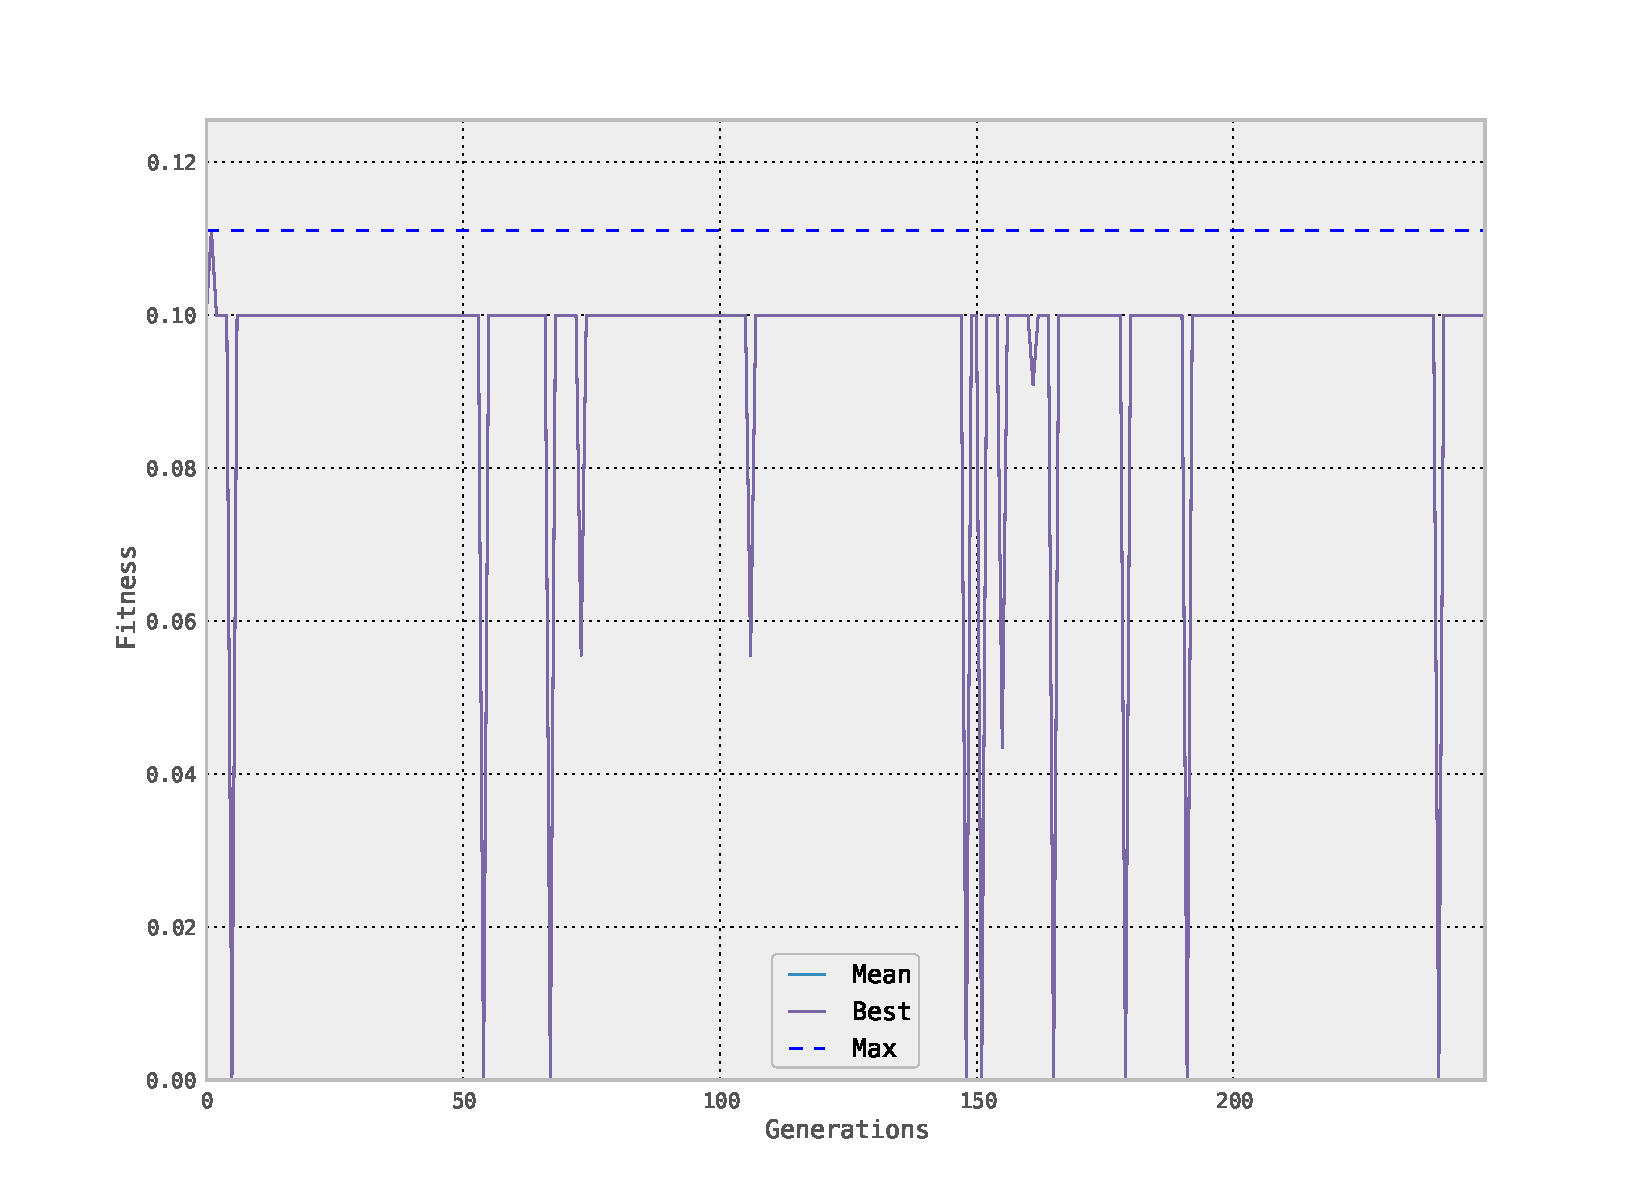
\includegraphics[scale =0.3] {images/section1/fitness_incremental_learning_update_ProportionalAnt.pdf}
	\label{fig:subfig11}
}
\subfigure[Pheromones per edge]{
	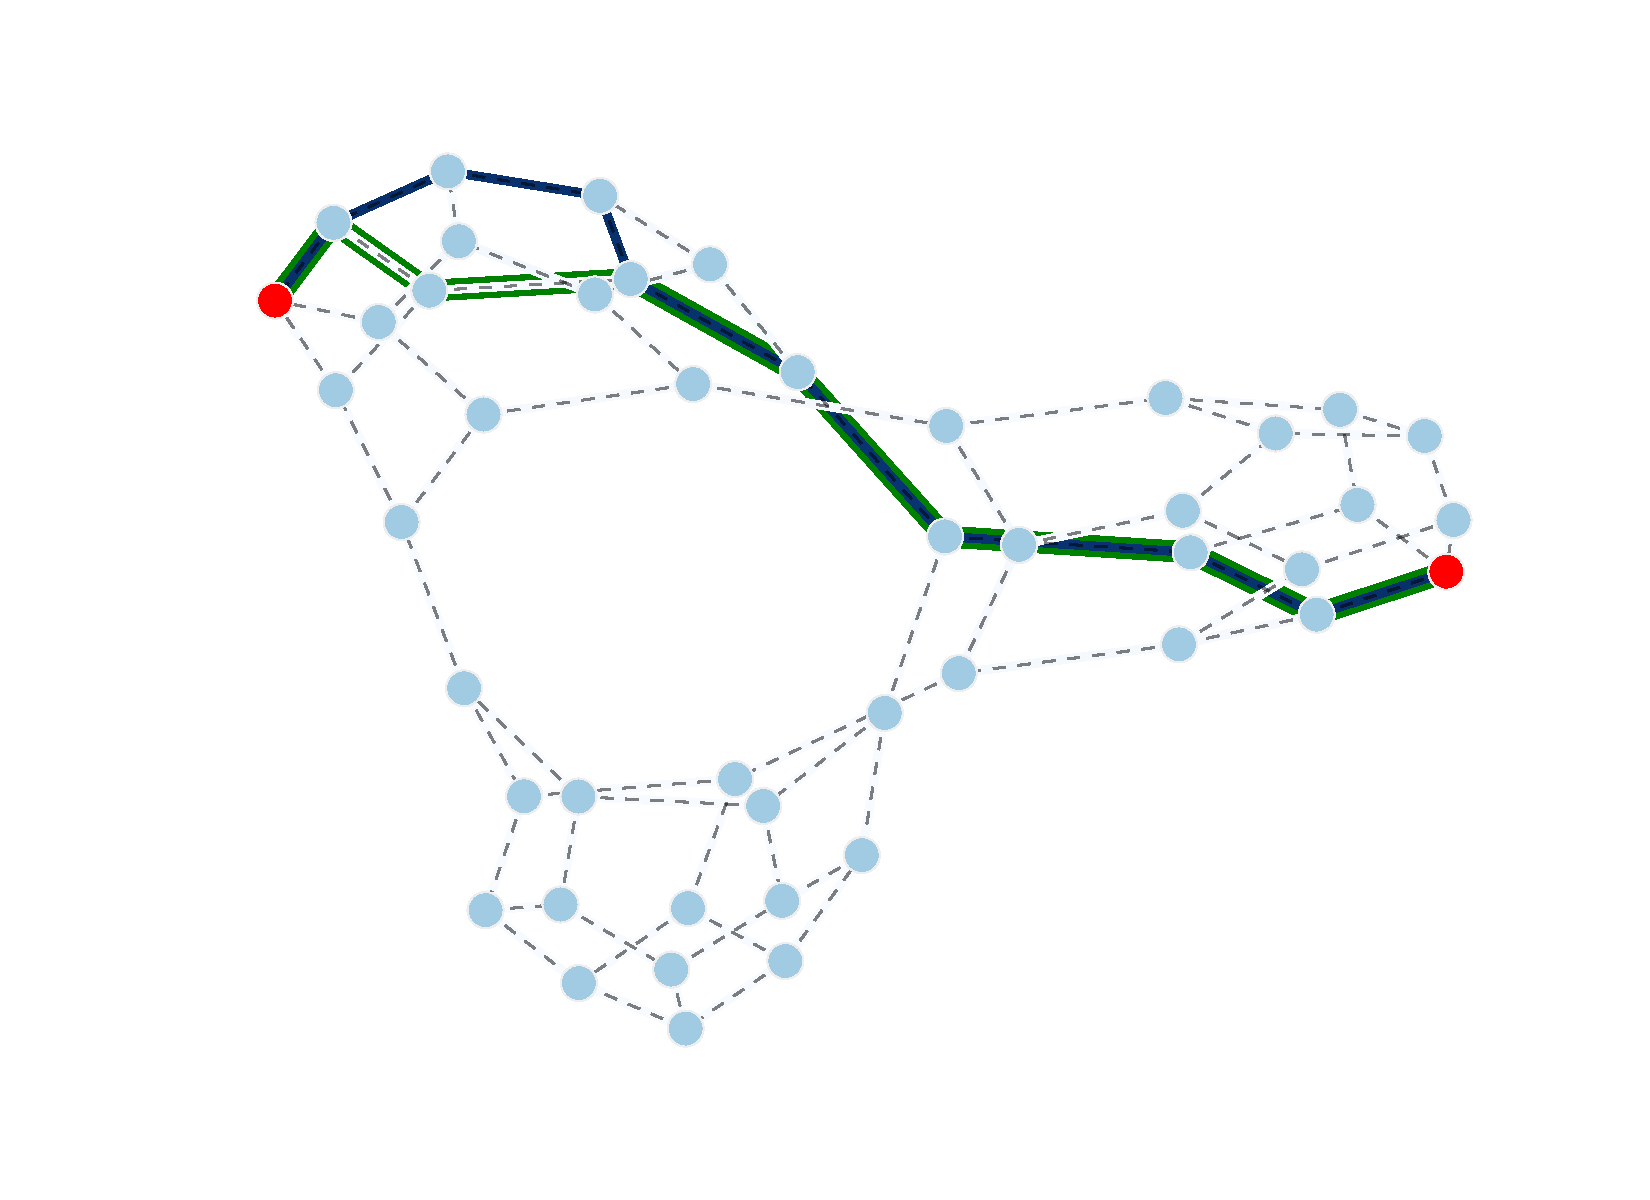
\includegraphics[scale =0.3] {images/section1/pheromones_incremental_learning_update_ProportionalAnt.pdf}
	\label{fig:subfig12}
}
%\caption[Optional caption for list of figures]{Caption of subfigures \subref{fig:subfig1}, \subref{fig:subfig2}}
\label{fig:fig1}
\end{figure}







\newpage
\subsection{Conclusions}
As the results shows, we can see that The Linear BM model + Binary, we perform a huge exploration reaching the best path randomly. With a The Linear BM model + Proportional the method is able to make a bias to the best one. The incremental learning algorithm works perfectly to reaching the optimal path.